\documentclass[../reportesINE.tex]{subfiles}

\usepackage{amssymb} %viñetas personalizadas

\begin{document}
\subsection{Descripción del funcionamiento}

\subsubsection{Acceso al módulo}
Sólo aquellos usuario con cuenta institucional y que estén dados de alta en el sistema con rol \textit{CONSULTA} podrán acceder al módulo de consulta. Se requiere de una computadora con conexión a internet para el acceso. 

\subsubsection{Manual de funcionalidad}
\begin{itemize}
\item Através de cualquier navegador web, desde cualquier computadora con conexión a internet, entrar a la liga: \textbf{https://sidj.ine.mx/}. \textit{Imagen \ref{fig:ej1}}

\begin{figure}[h]
  \centering
  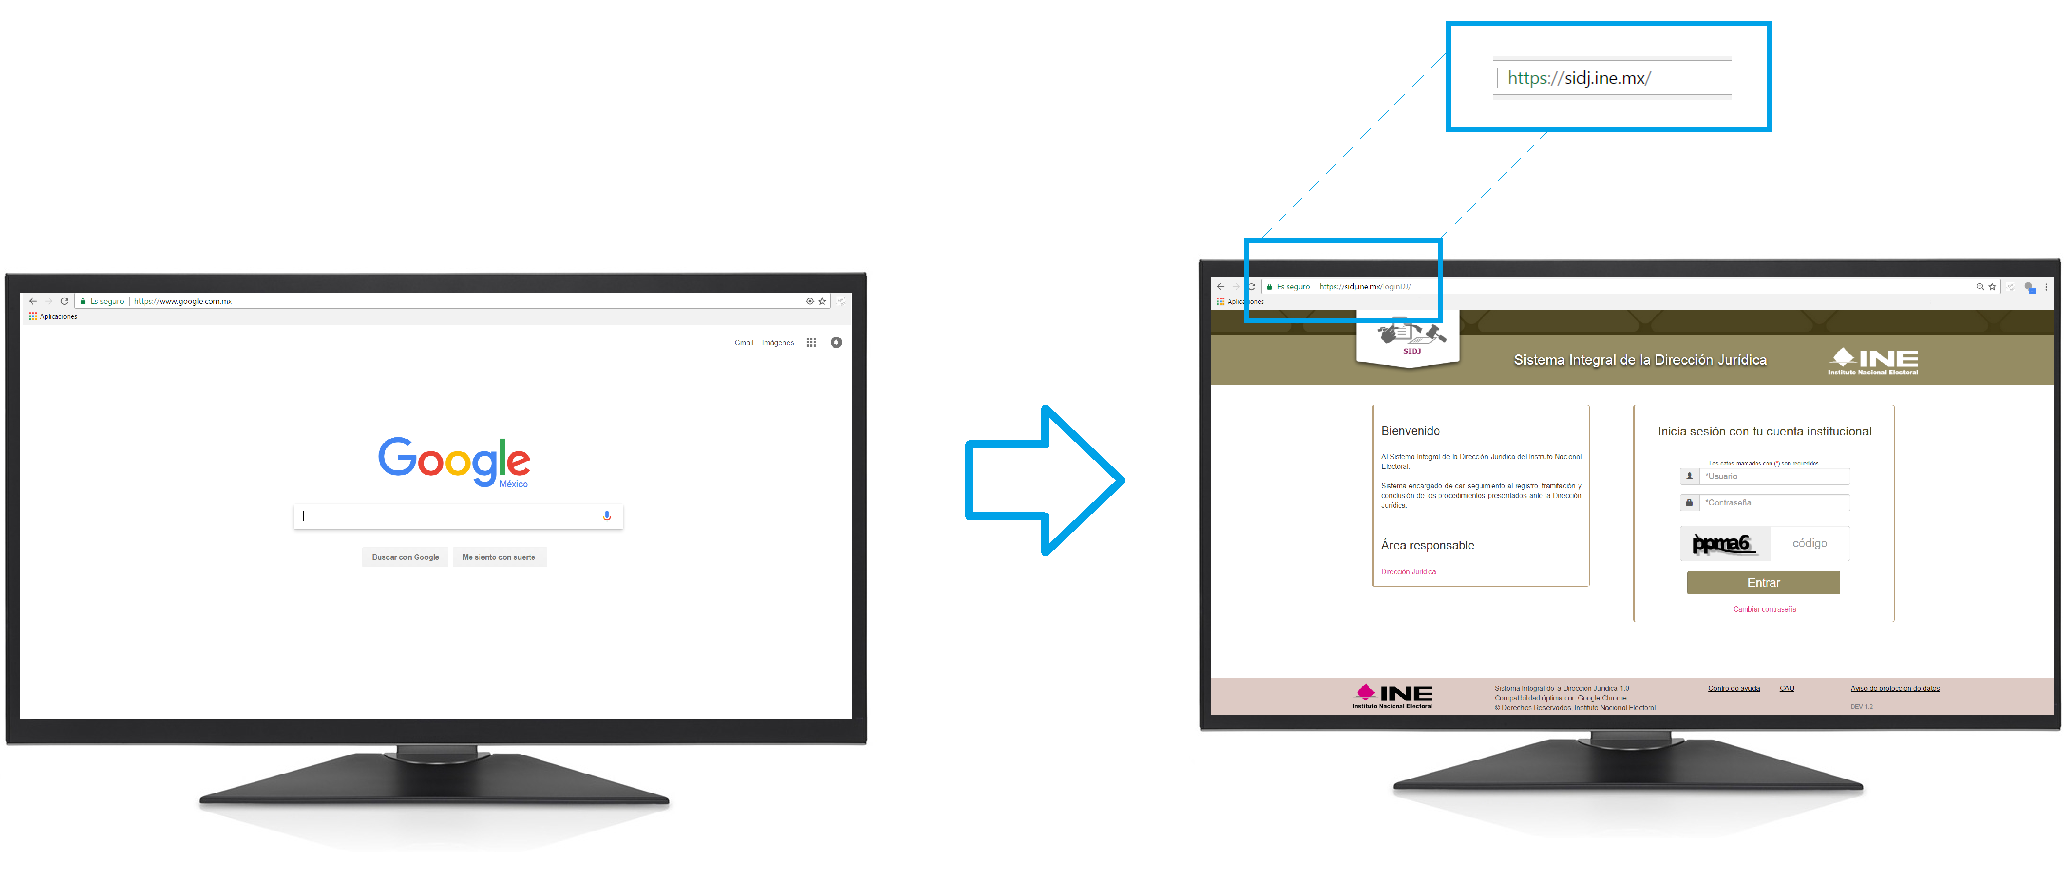
\includegraphics[width=\linewidth]{ejemplo/ej1.png}
  \caption{Acceso al Sistema de la Dirección Jurídica.}
  \label{fig:ej1}
\end{figure}

\item Presentar credenciales correspondientes (usuario y contraseña), teclear código de seguridad y presionar el botón \textbf{Entrar}. \textit{Imagen \ref{fig:ej2}}

\begin{figure}[h]
  \centering
  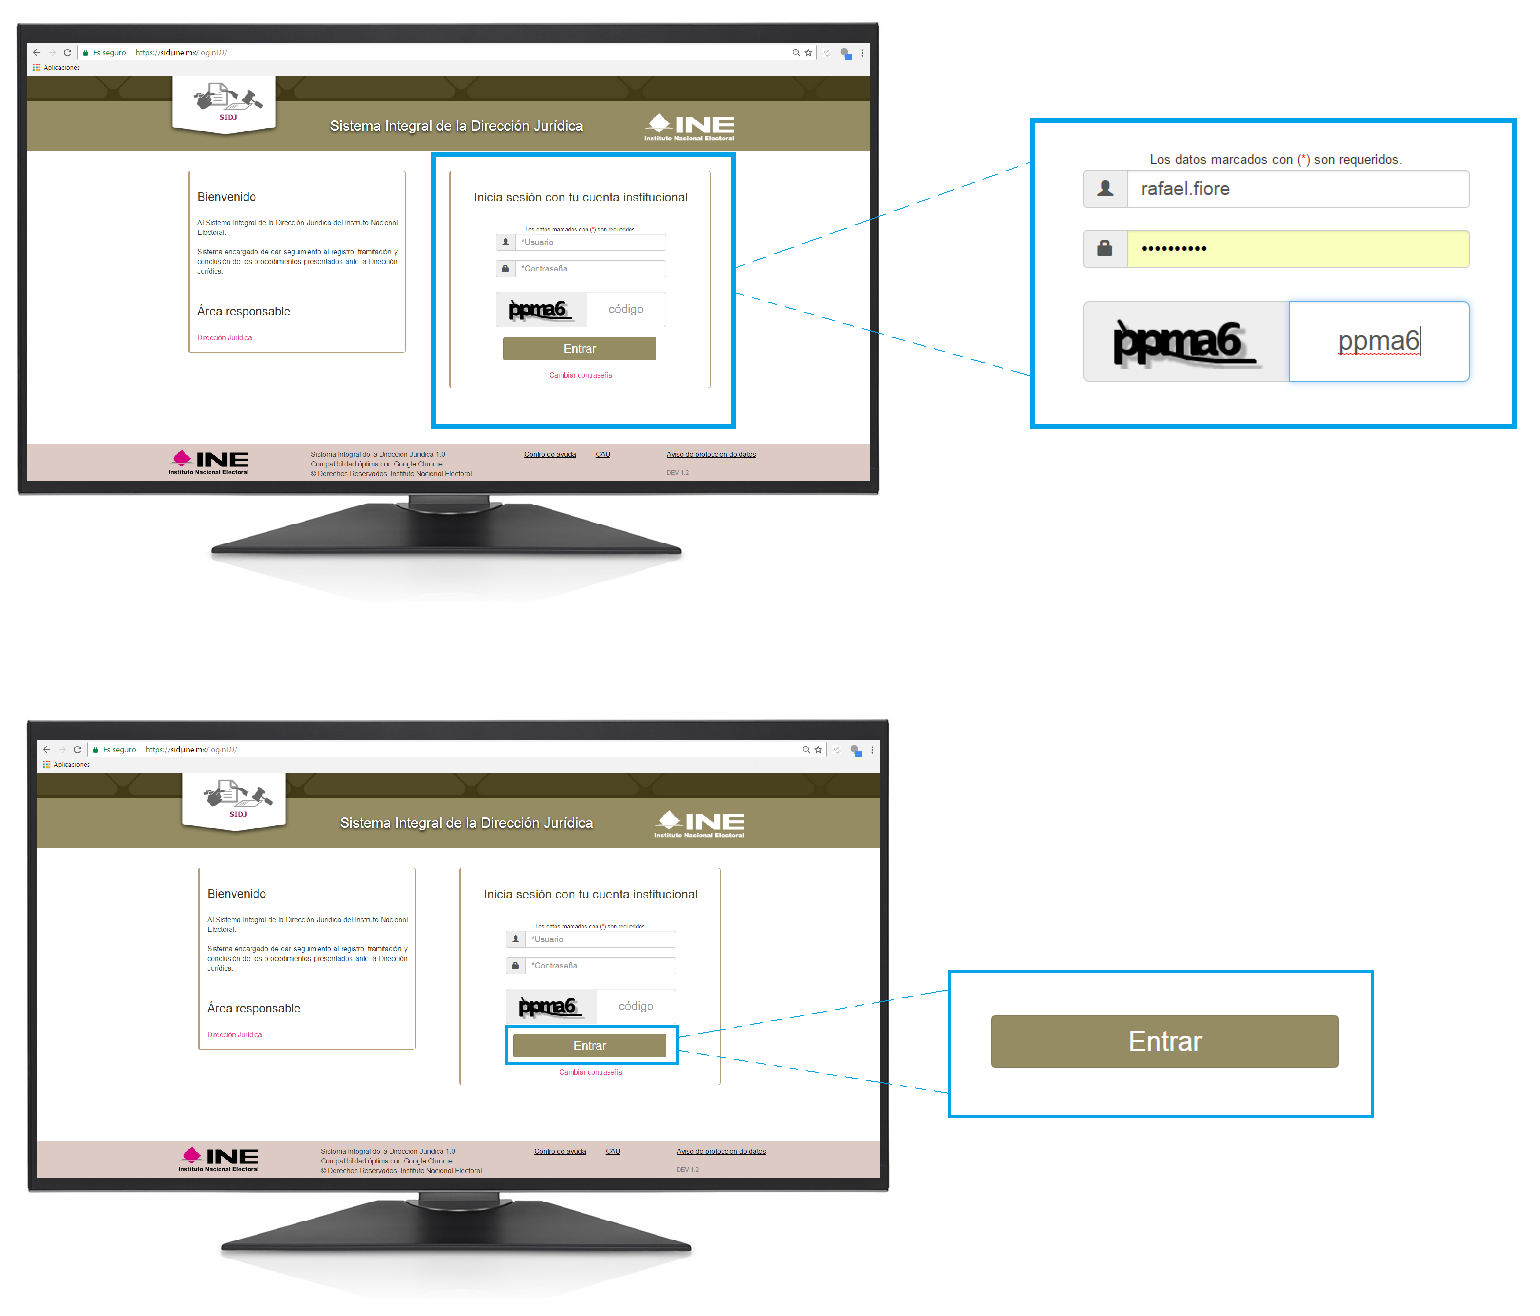
\includegraphics[width=\linewidth]{ejemplo/ej2.png}
  \caption{Ejemplo de  credenciales para el acceso al Sistema de la Dirección Jurídica.}
  \label{fig:ej2}
\end{figure}

\item Si se presenta la pantalla de \textbf{Seleccionar módulo}, seleccionar el módulo \textbf{CONSULTA}, esta pantalla sólo se mostrará en caso de que se tengan permisos adicionales a los de \textit{CONSULTA} en el sistema, de lo contrario se direccionara automáticamente a la pantalla del siguiente punto. \textit{Imagen \ref{fig:ej3a}}

\begin{figure}[h]
  \centering
  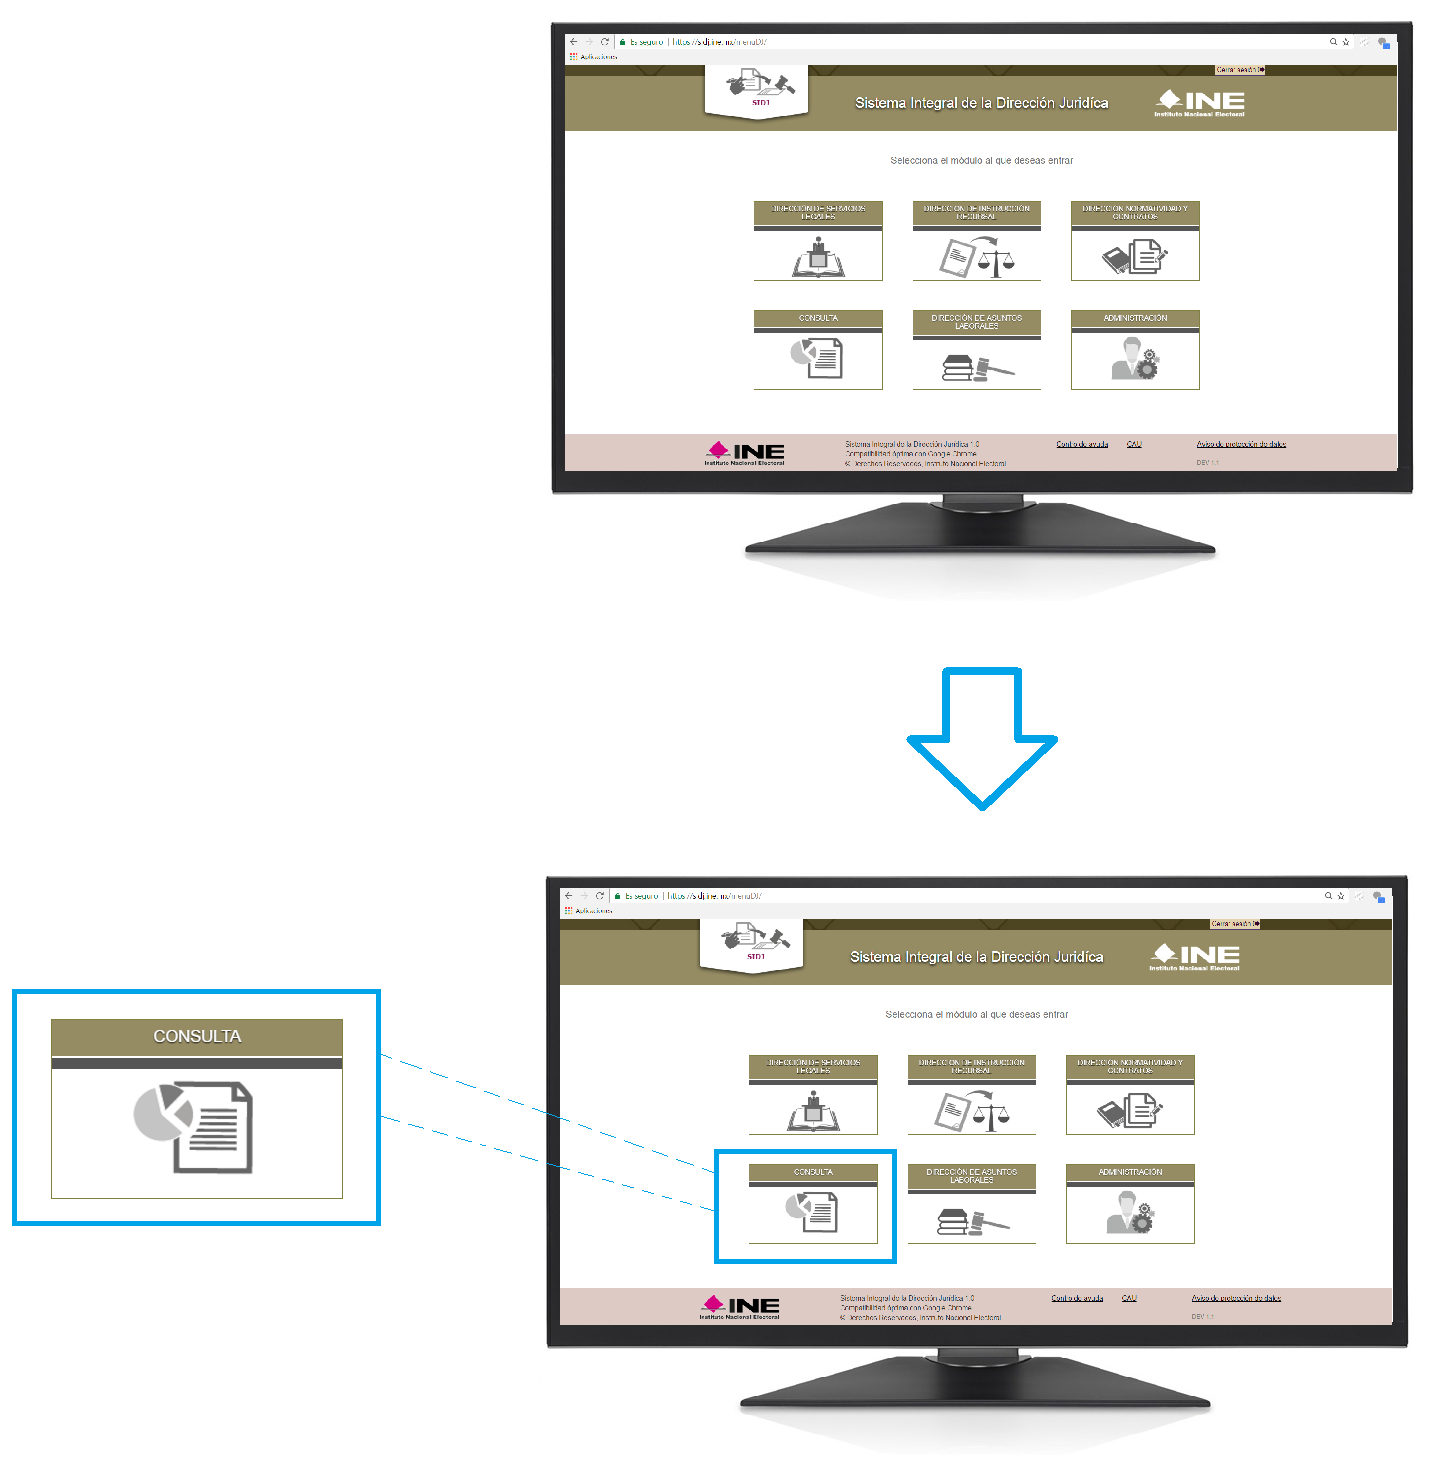
\includegraphics[width=\linewidth]{ejemplo/ej3a.png}
  \caption{Pantalla donde se muestran los módulos del Sistema de la Dirección Jurídica.}
  \label{fig:ej3a}
\end{figure}

\item En parte superior se encuentra un menú (franja de color vino) con las opciones disponibles para la \textit{CONSULTA} de datos, seleccionar la opción de \textbf{Reportes}. \textit{Imagen \ref{fig:ej3b}}

\begin{figure}[h]
  \centering
  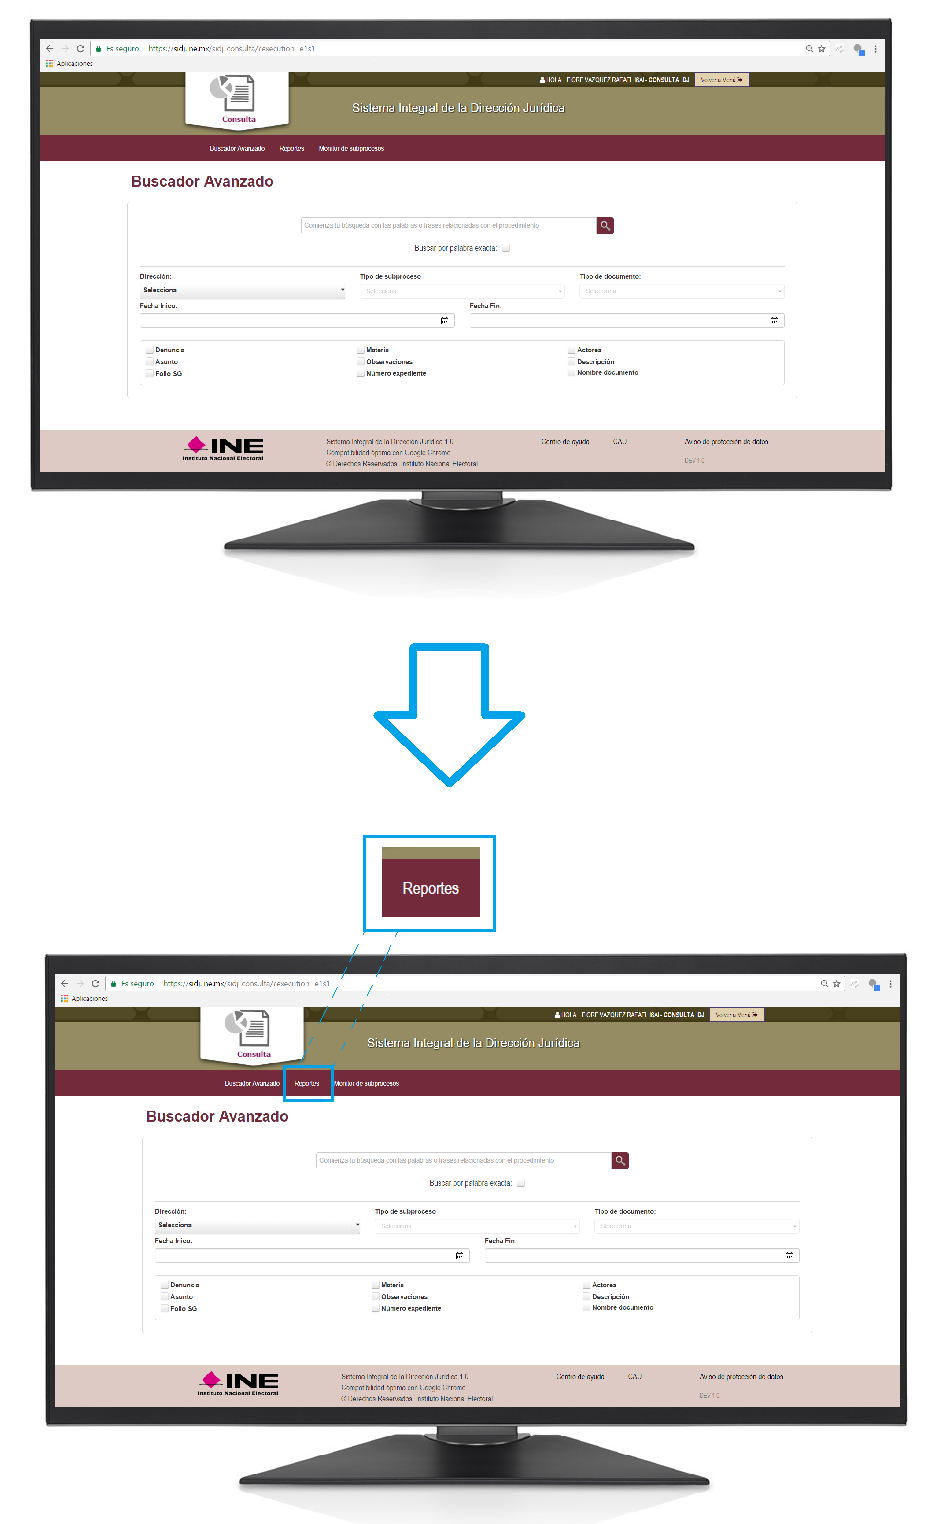
\includegraphics[width=\linewidth]{ejemplo/ej3b.png}
  \caption{Pantalla inicial para usuarios con rol CONSULTA en el Sistema de la Dirección Jurídica.}
  \label{fig:ej3b}
\end{figure}

\item Se muestra un menú con los sistemas de la \textit{Dirección Jurídica}, seleccionar el sistema deseado. \textit{Imagen \ref{fig:ej4}}

\begin{figure}[h]
  \centering
  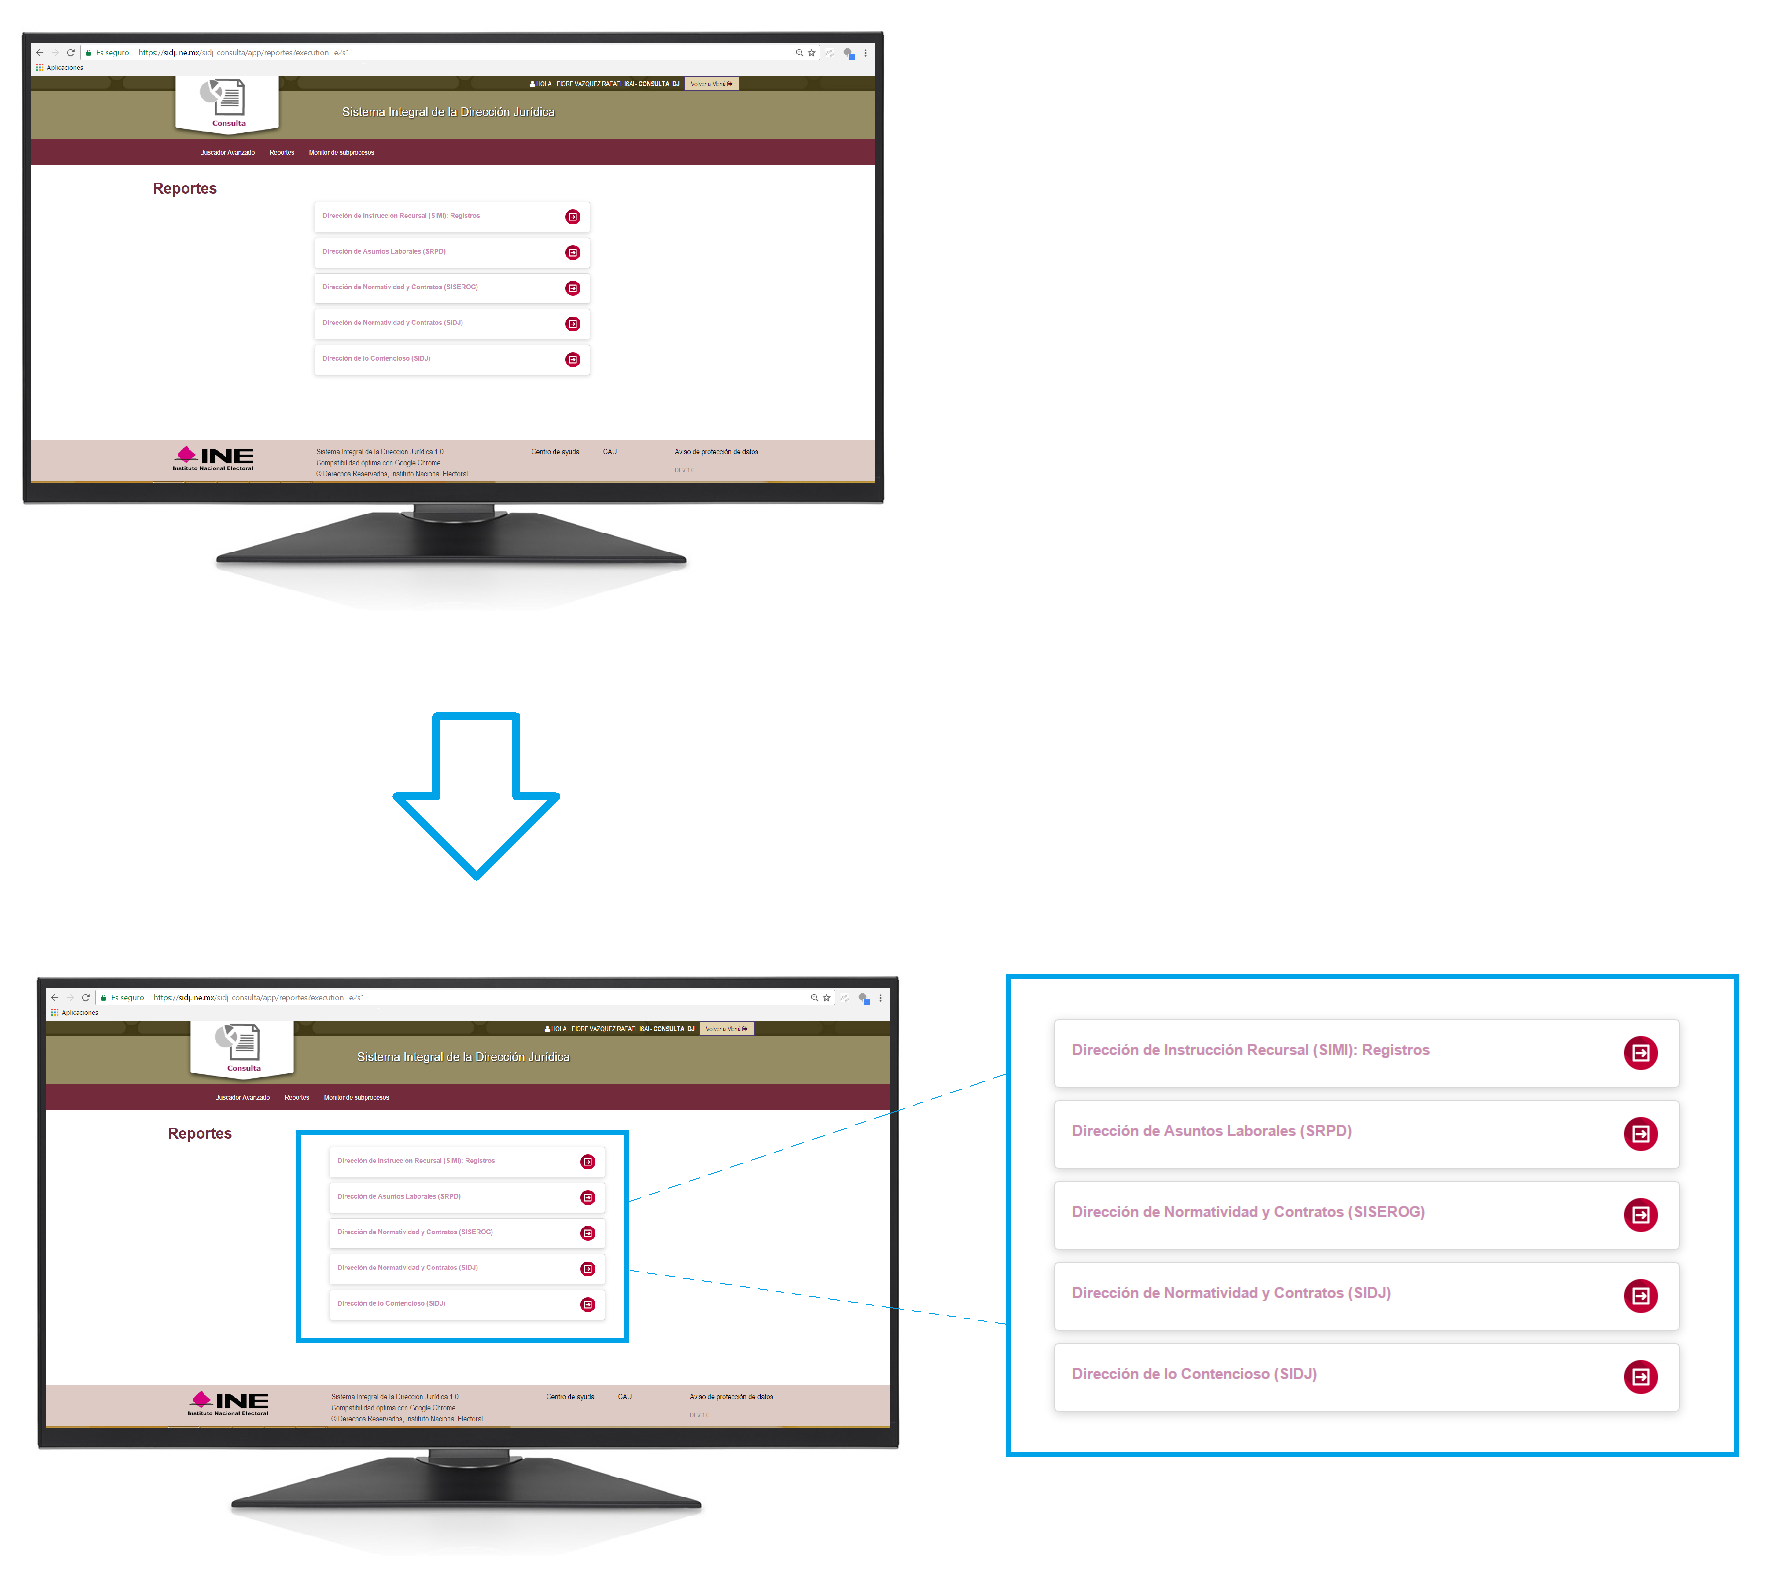
\includegraphics[width=\linewidth]{ejemplo/ej4.png}
  \caption{Menú de seleccion de sistemas de la Dirección Jurídica disponibles para consulta.}
  \label{fig:ej4}
\end{figure}

\item En la sección de filtros se encuentran las columnas disponibles para el reporte, para seleccionar una columna activar el \textit{checkbox} que se encuentra a la izquierda. \textit{Imagen \ref{fig:ej5a}}
Se despliega el filtro correspondiente a esa columna, el sistema cuenta con tres tipos de filtros: \textit{Imagen \ref{fig:filtros}}
\begin{itemize}
\item Filtro de búsqueda por palabra o frase: teclear la palabra o frase en la línea debajo del título de la columna.
\item Filtro de búsqueda exacta: se despliega debajo del título de la columna una lista con opciones para el filtrado.
\item Filtro de búsqueda por rango de fechas: se despliega dos calendarios debajo del título de la columna, si sólo se selecciona una fecha en el calendario de la izquierda el filtro será por fecha exacta si ambos calendarios contienen una fecha el filtro será por el rango marcado por ambas fechas. 
\end{itemize}

\begin{figure}[h]
  \centering
  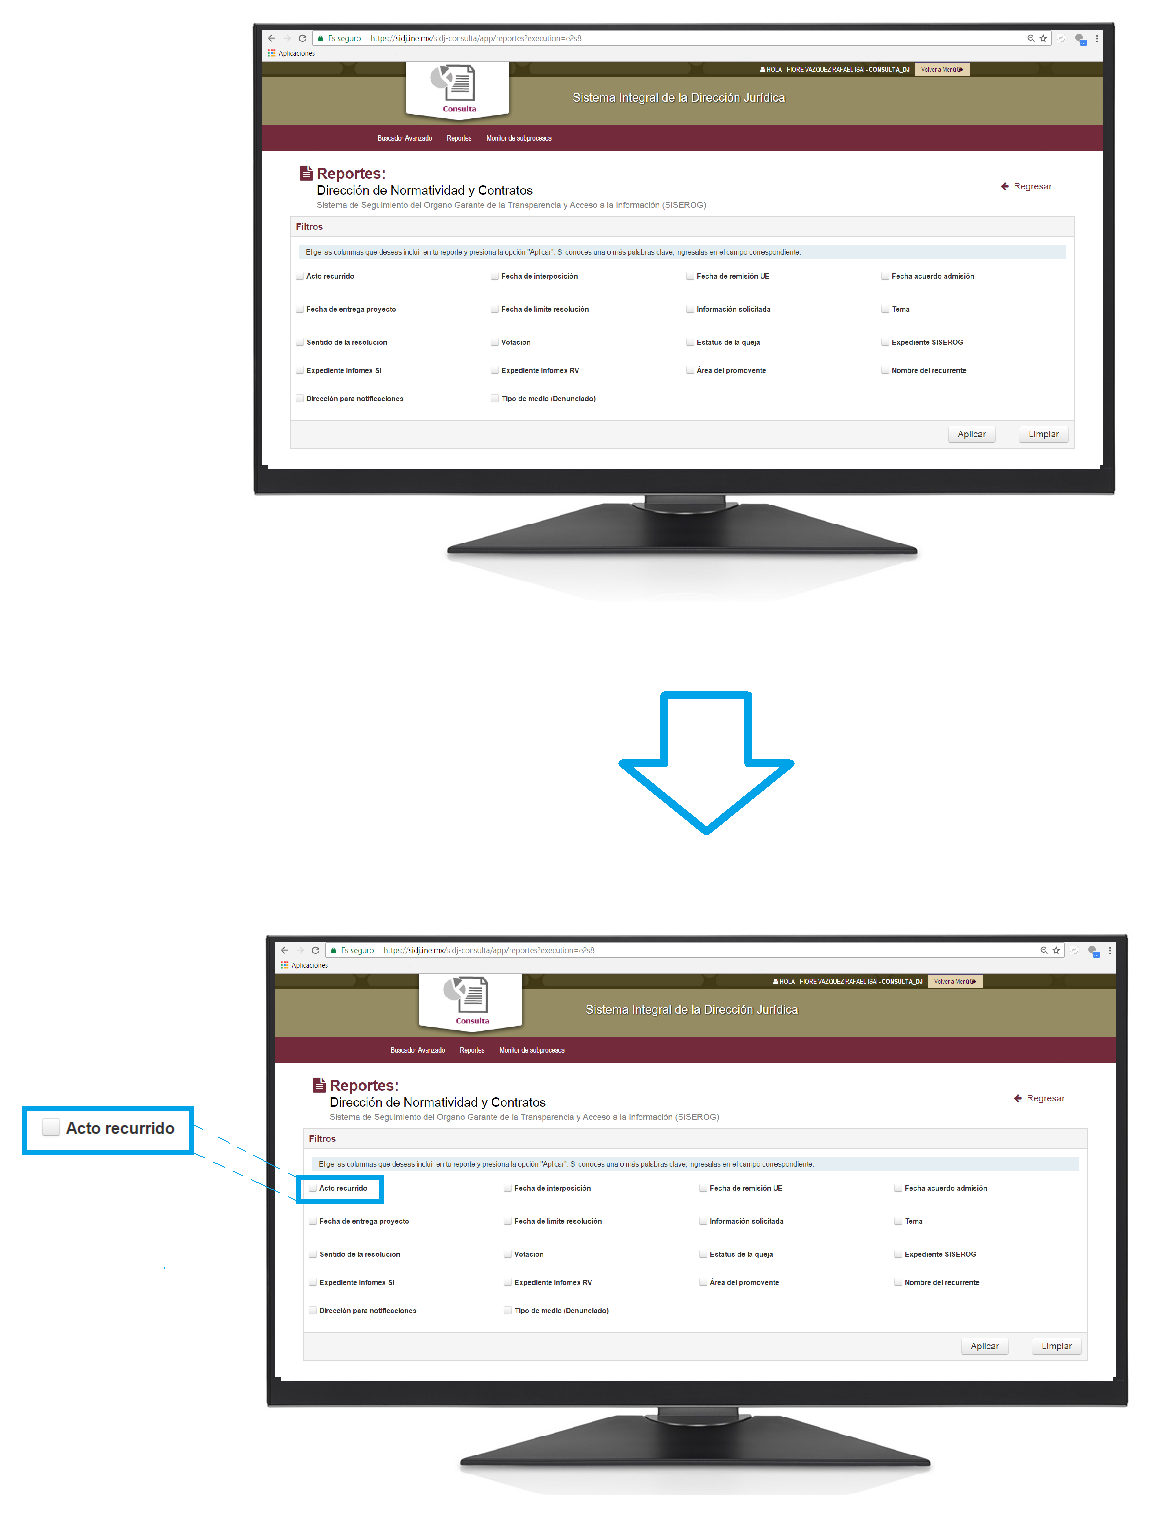
\includegraphics[width=\linewidth]{ejemplo/ej5a.png}
  \caption{Ejemplo de pantalla para consulta.}
  \label{fig:ej5a}
\end{figure}

\begin{figure}
  \centering
  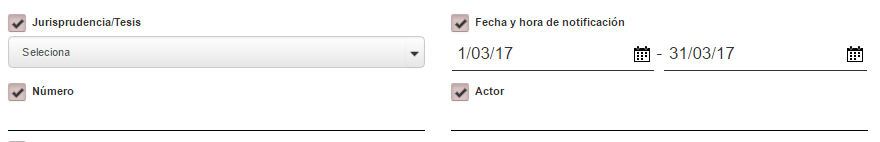
\includegraphics[width=\linewidth]{ejemplo/filtros.PNG}
  \caption{Filtros disponibles para consulta.}
  \label{fig:filtros}
\end{figure}

\item Si no se desea agregar filtro simplemente se dejan en blanco, así la columna aparecerá en el reporte sin ningún tipo de filtro. Una vez que se han seleccionado las columnas deseadas con o sin filtros, presionar el botón de \textbf{Aplicar}. \textit{Imagen \ref{fig:ej5b}}

\begin{figure}[h]
  \centering
  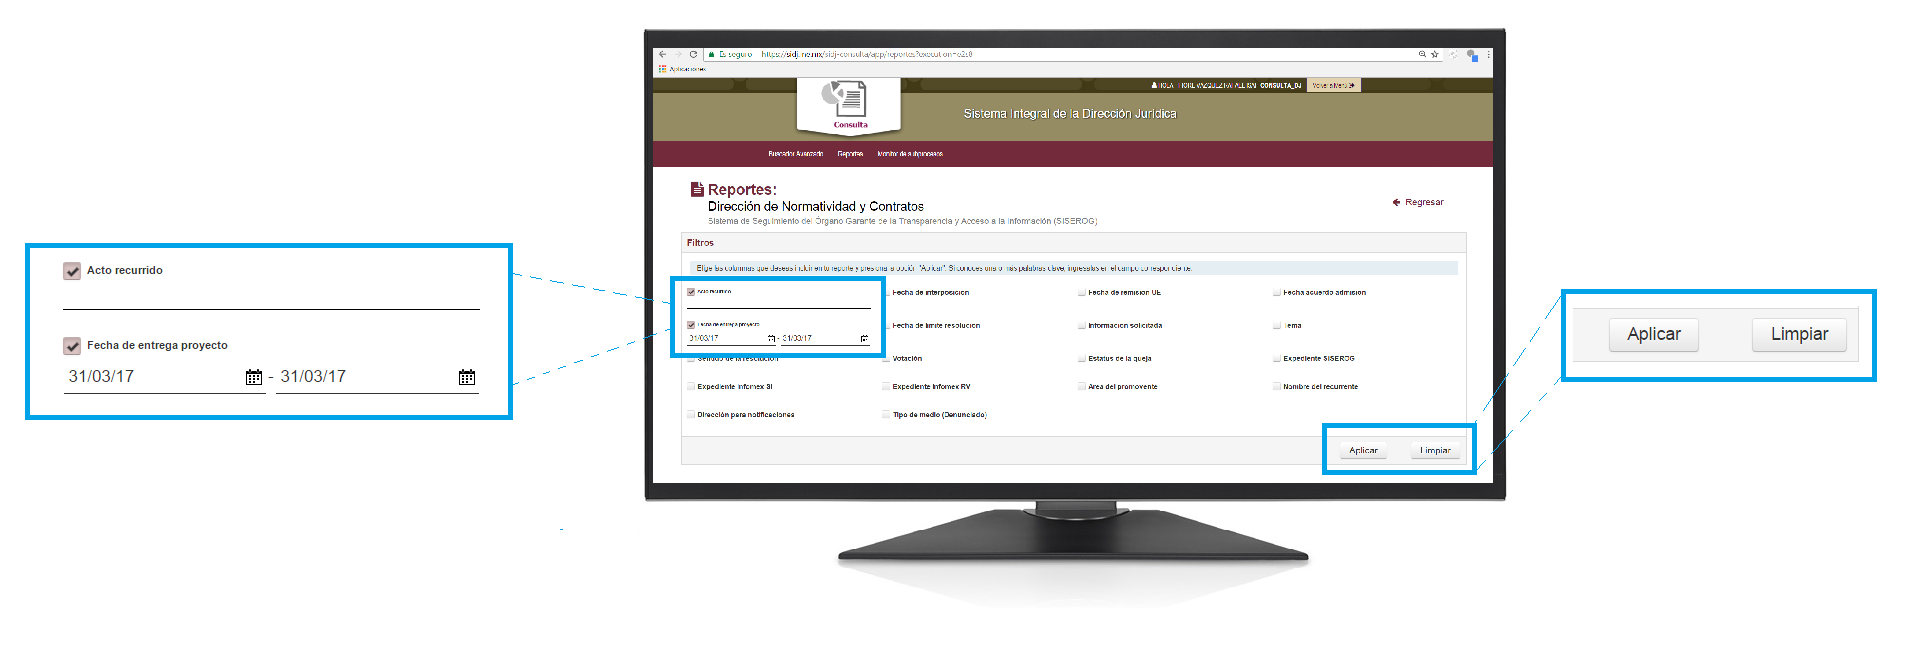
\includegraphics[width=\linewidth]{ejemplo/ej5b.png}
  \caption{Ejemplo de pantalla con filtros seleccionados para consulta.}
  \label{fig:ej5b}
\end{figure}

\item Aparecerá una vista previa del reporte generado. En la parte superior de la vista se tiene como disponible la opción de \textbf{Descarga}. \textit{Imagen \ref{fig:ej5c}}

\begin{figure}[h]
  \centering
  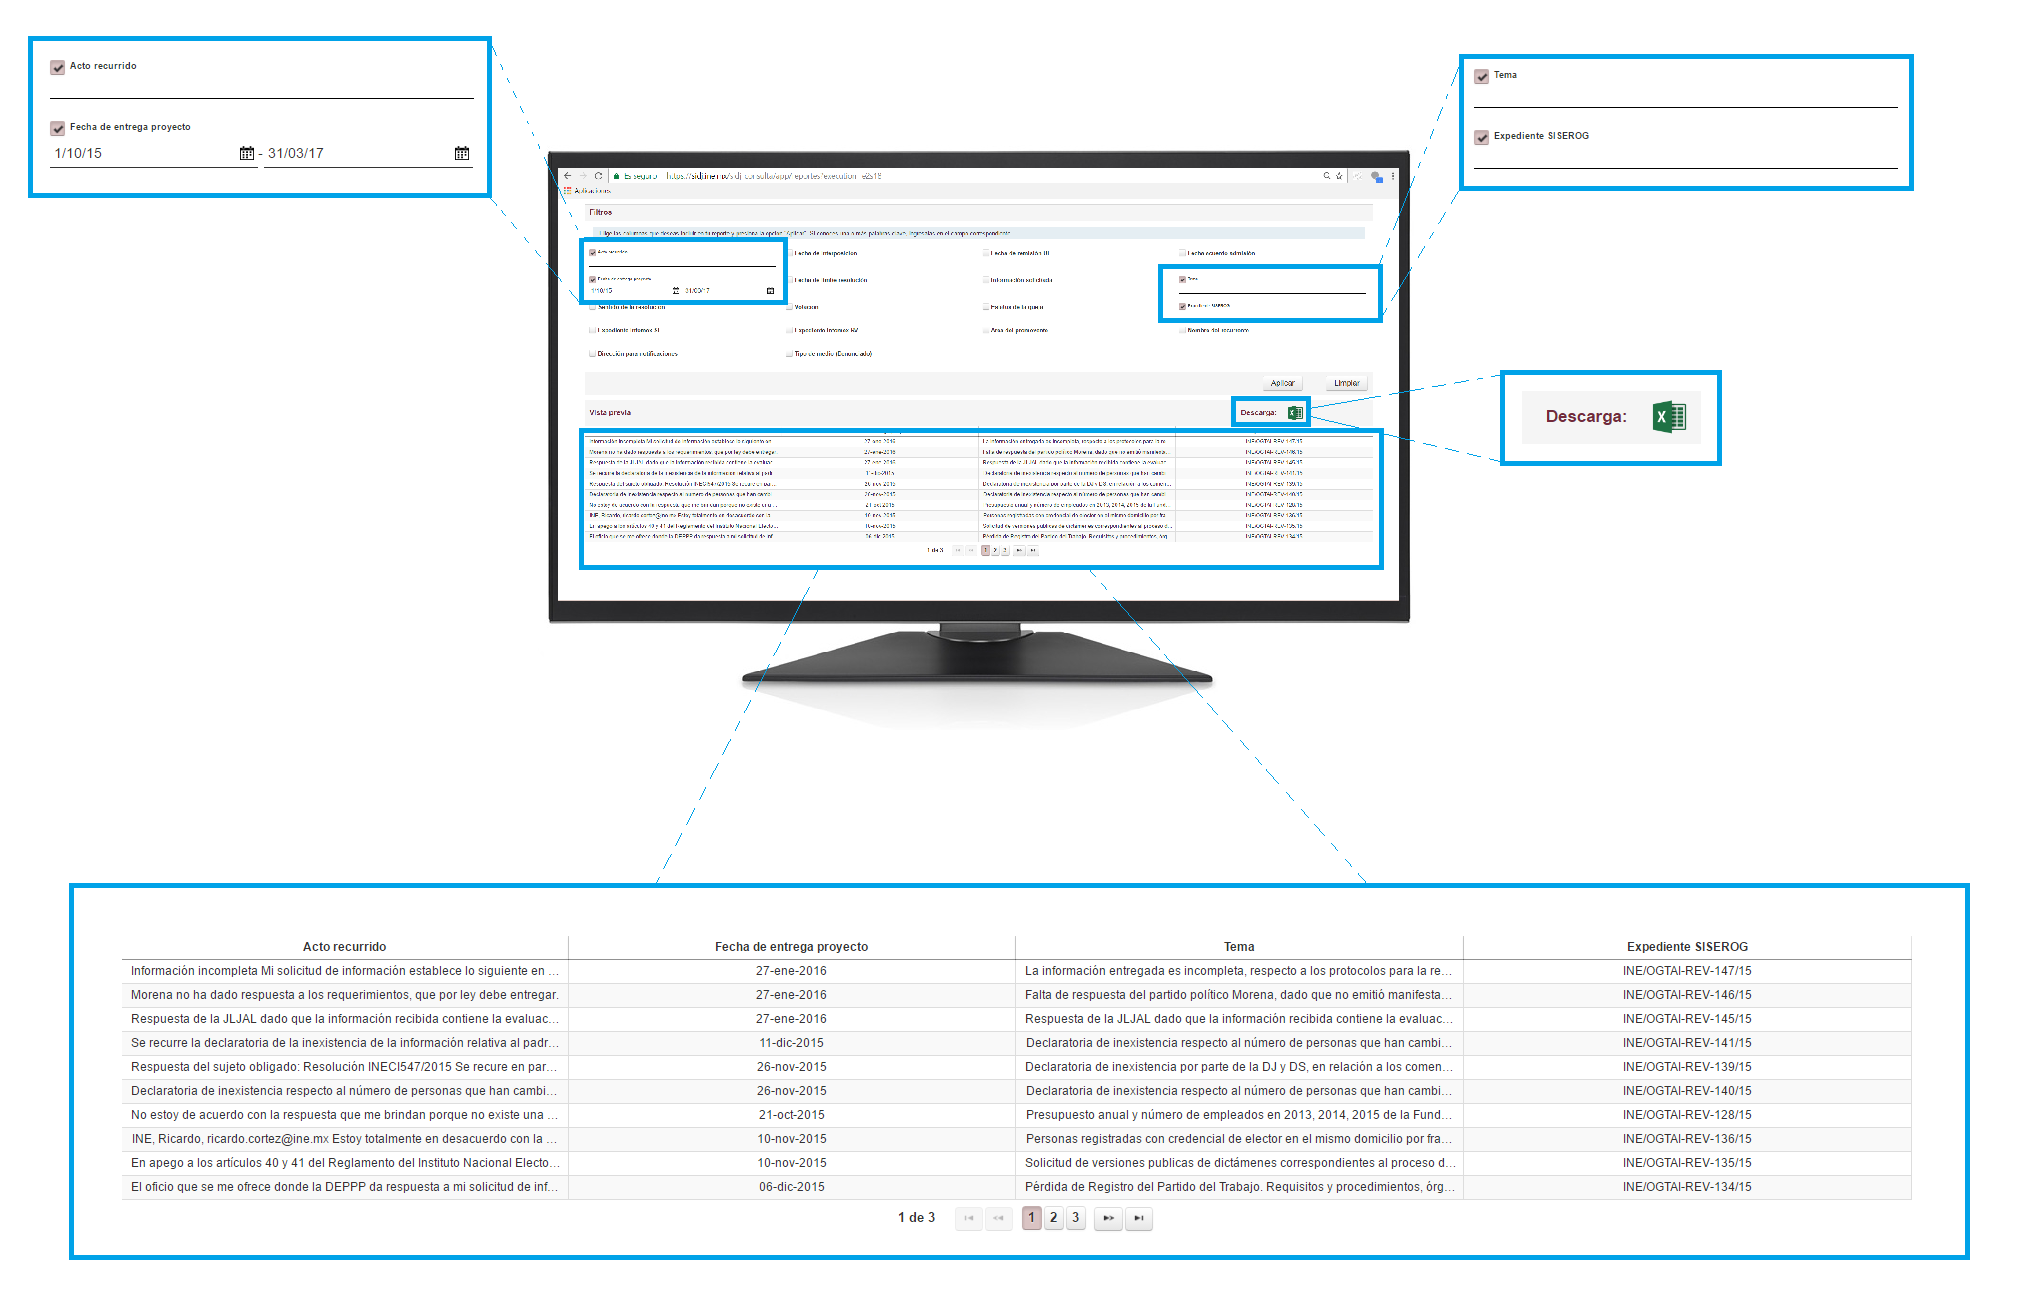
\includegraphics[width=\linewidth]{ejemplo/ej5c.png}
  \caption{Ejemplo de pantalla con vista previa para consulta.}
  \label{fig:ej5c}
\end{figure}

\item Para generar excel con la información de la vista previa presionar el icono correspondiente y la descarga del archivo es automática. \textit{Imagen \ref{fig:ej6}}

\begin{figure}[h]
  \centering
  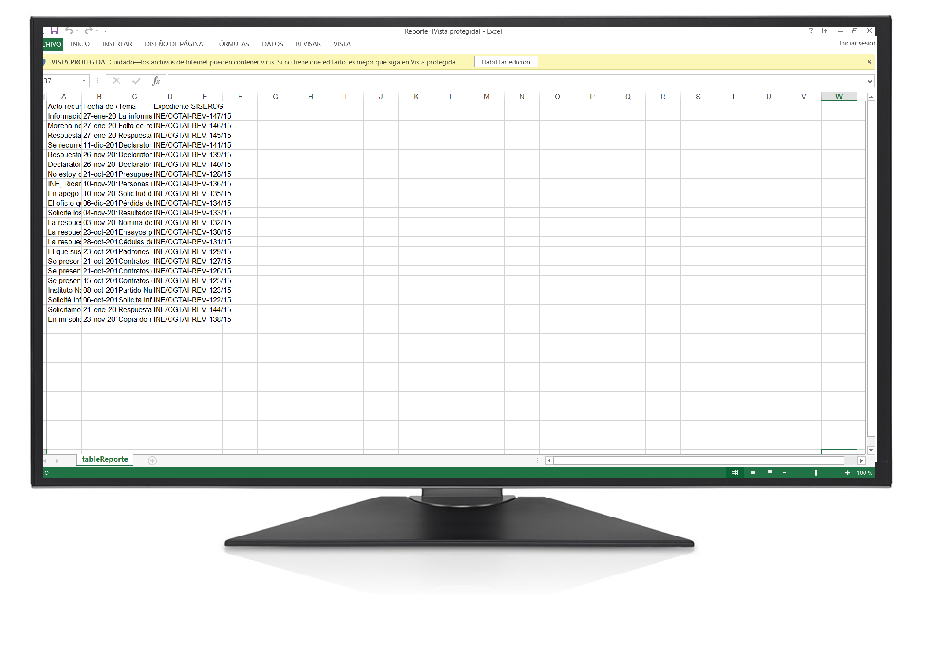
\includegraphics[width=\linewidth]{ejemplo/ej6.png}
  \caption{Ejemplo de excel generado a partir del módulo de consulta.}
  \label{fig:ej6}
\end{figure}

\end{itemize}

\subsubsection{Pruebas: Módulo de consulta y reportes}

\begin{itemize}
\item[$\square$]  Descripción de la prueba
\item[$\square$]  #Pruebas realizadas
\item[$\square$]  Errores
\item[$\square$]  Observaciones/Comentarios
\end{itemize}
  

\end{document}